\section{mo\-Cool\-Sched Class Reference}
\label{classmo_cool_sched}\index{moCoolSched@{moCoolSched}}
This class gives the description of a cooling schedule.  


{\tt \#include $<$mo\-Cool\-Sched.h$>$}

Inheritance diagram for mo\-Cool\-Sched::\begin{figure}[H]
\begin{center}
\leavevmode
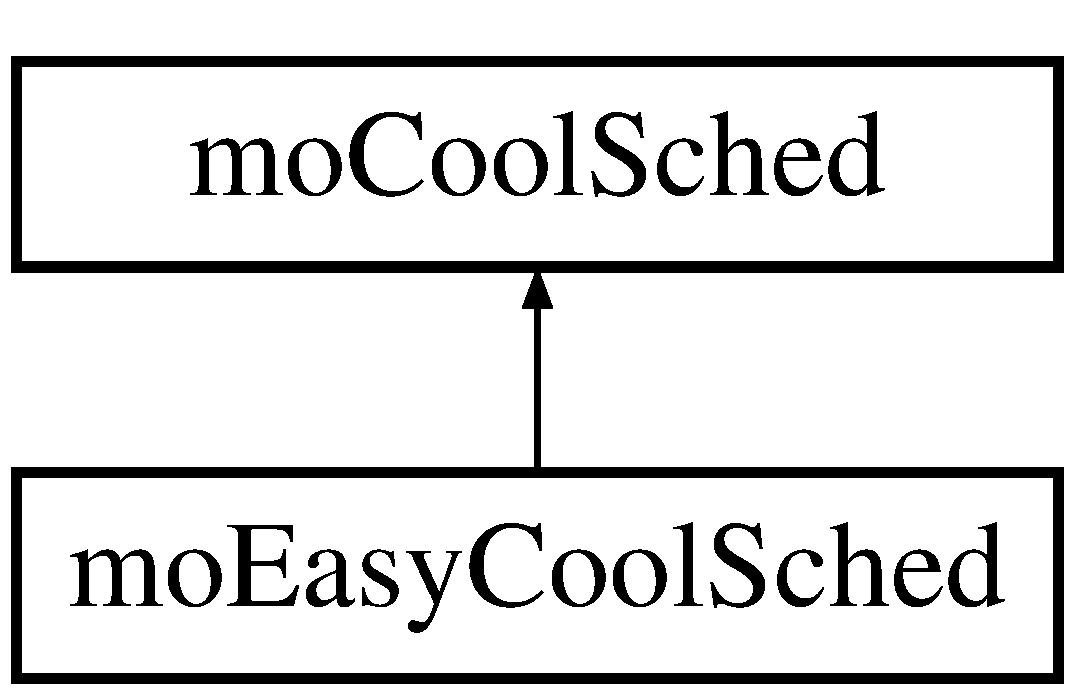
\includegraphics[height=2cm]{classmo_cool_sched}
\end{center}
\end{figure}


\subsection{Detailed Description}
This class gives the description of a cooling schedule. 

It is only a description... An object that herits from this class is needed to be used in a {\bf mo\-SA}{\rm (p.\,\pageref{classmo_s_a})}. See {\bf mo\-Easy\-Cool\-Sched}{\rm (p.\,\pageref{classmo_easy_cool_sched})} for example. 



Definition at line 22 of file mo\-Cool\-Sched.h.

The documentation for this class was generated from the following file:\begin{CompactItemize}
\item 
mo\-Cool\-Sched.h\end{CompactItemize}
